\section{Background}
\label{sec:Background}
In this section, we first briefly introduce the Amazon Marketplace. Then, we focus on the data features on the markets, that effect to algorithmic repricing, including the offers of 3P merchants, the BuyBox concept, and finally the scaled data, collected from the Amazon Web Services (AWS).

\subsection{The Amazon Marketplace}
\label{sec:amzintro}
%% Talk a bit about Amazon online marketplace
The Amazon Marketplace is one of the most well-known marketing channels for online retailers. 
It is an e-commerce platform, which enables  sellers to sell their products on its cloud markets. 
Started as a book seller but later Amazon (amazon.com) has expanded to sell varied categories of consumer 
items as well as its own electronic machinery. The Amazon has separate marketplaces for the United States, 
Australia, Brazil, Canada, China, France, Germany, India, Italy, Japan, Mexico, Netherlands, Spain, and the United Kingdom.

In 2015, Amazon surpassed Walmart to be the most valuable retailer in the United States \cite{kantor2015inside}. 
In 2017, it becomes one of the top 10 world's largest online marketplace with around 80 million worldwide members 
(refered to \textit{"Global Powers of Retailing 2017"} report {\footnote{\url{https://www2.deloitte.com/
content/dam/Deloitte/global/Documents/consumer-industrial-products/gx-cip-2017-global-powers-of-retailing.pdf}}). 
In the same year, the using Amazon mobile application also reached the peak of 41.50\% to become the top most 
popular mobile shopping app in the United States, this is illustrated by \textbf{Fig.\ref{fig:statistic}} 
(refered to www.statista.com {\footnote{\url{https://www.statista.com/statistics/579505/most-popular-
us-shopping-apps-ranked-by-reach/}}}). 

\begin{figure}[!h]
	\begin{center}
		\scalebox{0.27}{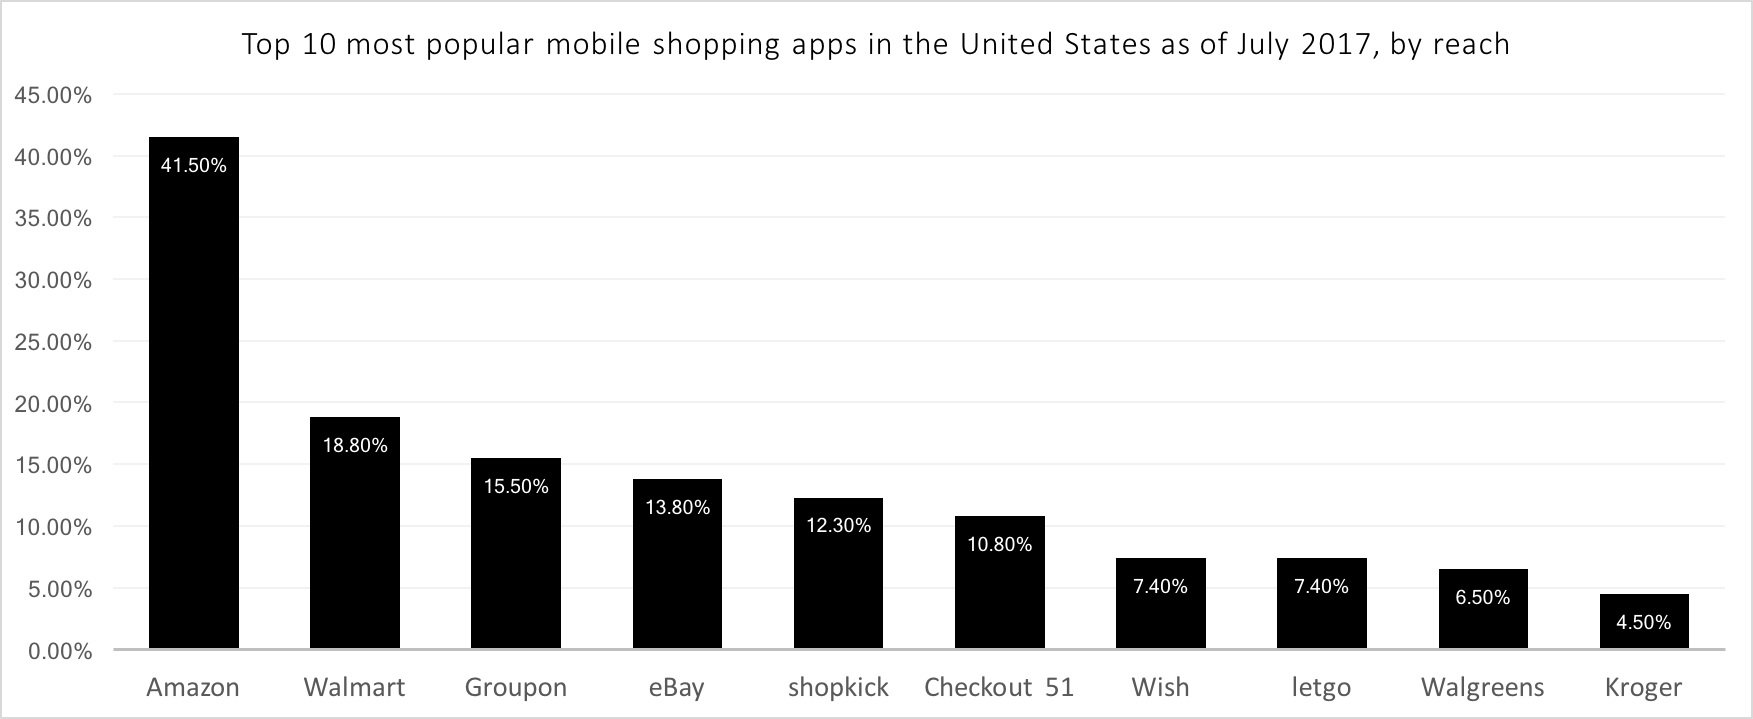
\includegraphics{fig6_statisticAMZ.png}}
	\end{center}
	\caption{\label{fig:statistic} Top 10 of most popular mobile shopping apps in the United States as of July 2017, by reach.}
\end{figure}
%%Talk more about amazon
%% FBA and FBM
%Goods purchased on Amazon from  sellers are either fulfilled by the merchant (FBM) or by Amazon (FBA). FBM sellers must keep items in their inventory, and must manage their shipping and customer service. Perversely, FBA sellers can store the goods in Amazon's fulfillment centers, while shipping and customer services are organized by Amazon. 

%% Amazon fee -> need to take advantage from repricing
%There are several Selling Fees for  retailers to put their products on Amazon Marketplace, including:
%\begin{enumerate}
%	\item \textbf{Per-item Fee}: When one product sells, Amazon collects the amount paid by the buyer (\$0.99/item sold, or sellers may become “Pro Merchants” with no fee)
%
%	\item \textbf{Referral Fee}:  sellers have to pay a referral fee on each product sold. The referral fees vary by category between 6\%-45\% of the total sale price. However, the enforcement of minimum referral fees is \$1-\$2/item.
%
%	\item \textbf{Closing Fee}: For each media product that is sold, Individual and Professional Sellers also pay a variable closing fee (\$1.80 per media product).
%
%	\item \textbf{High-Volume Listing Fee}: Amazon charges a monthly High-Volume Listing Fee based on the number of active offers for non-media products listed on Amazon (\$0.005 per product).
%
%	\item \textbf{Refund Administration Fee}: It is the lesser of \$5.00 or 20\% of the applicable Referral Fee if a seller refunds a customer for an order for which that seller has already received payment.
%\end{enumerate}

%\subsubsection{Third-party Sellers and FBA}. In addition to acting as a merchant, Amazon also functions as a marketplace for third parties. Amazon claims to have 2M Third-Party () sellers worldwide who sold 2B items in 2014, representing 40\% of all items sold via the website.  sellers can opt to handle logistics (inventory, shipping, returns, etc.) themselves, or they can join the Fulfilled By Amazon (FBA) program, in which case Amazon handles all logistics.

\subsection{The BuyBox}
\label{sec:buybox}
%% What is winner BuyBox?
The Amazon BuyBox is definitely the most important element to sellers in Amazon Marketplace. 
It is the box from the right of the product page which contains the \textit{"Add to Basket"} 
or \textit{"Add to Cart"} button. \textbf{Fig.\ref{fig:buyboxexample}}, an example BuyBox, 
shows that winning the BuyBox is critical for generating sales. The BuyBox contains the price 
of the product, shipping information, the name of the seller, and a button to purchase the product.
 When customers click the button, they are buying the product from only one merchant who is the BuyBox 
 winner. The winner gets more chance to sell their items by getting the prominent position in product's 
 page , while the other competitors are relegated to the bottom section with a lower priority. Amazon 
 themselves admit that around 82\% of purchases are made through the BuyBox \cite{taftamazon}. 

\begin{figure}[!h]
	\begin{center}
		\scalebox{0.40}{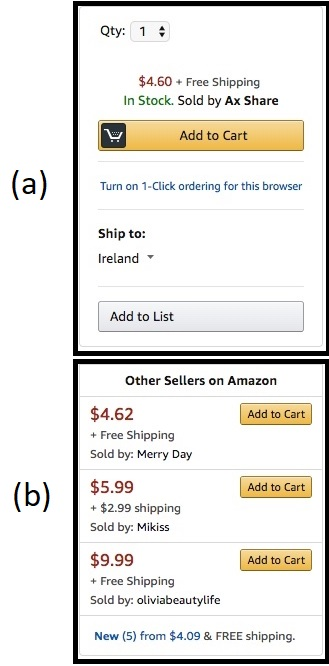
\includegraphics{fig1_buybox.png}}
	\end{center}
	\caption{\label{fig:buyboxexample}In the Amazon's product page, the products of the BuyBox 
		winner can be highlight effectively in the BuyBox (a), while the other competitors get lower 
		positions (b).}
\end{figure}


%% Why is it important?
However, multiple sellers can offer the same product in Amazon Marketplace. If more than one eligible seller offers a product, they may compete for the BuyBox position. \textbf{Fig.\ref{fig:exampleoffer}} is an example of one product's auction provided by many competitors with different information, prices, deliveries, and conditions. Every time one seller changes the price of a their product, the BuyBox winner is re-assigned by Amazon. 

Amazon has a convoluted algorithm to determine which seller gets the prime location on the BuyBox. Understanding the BuyBox algorithm is essential, because it may help sellers choose better pricing strategies for their next auctions.  Amazon has a notation about the features which are used by the BuyBox algorithm \cite{amazon17}, but it is uncertain whether the feature list is complete, or what the important weights of the features are. Because winning the BuyBox is so critical for making sales on Amazon,  sellers may use dynamic pricing strategies that give them an advantage to be chosen by the BuyBox algorithm.

\begin{figure}[!h]
	\begin{center}
		\scalebox{0.25}{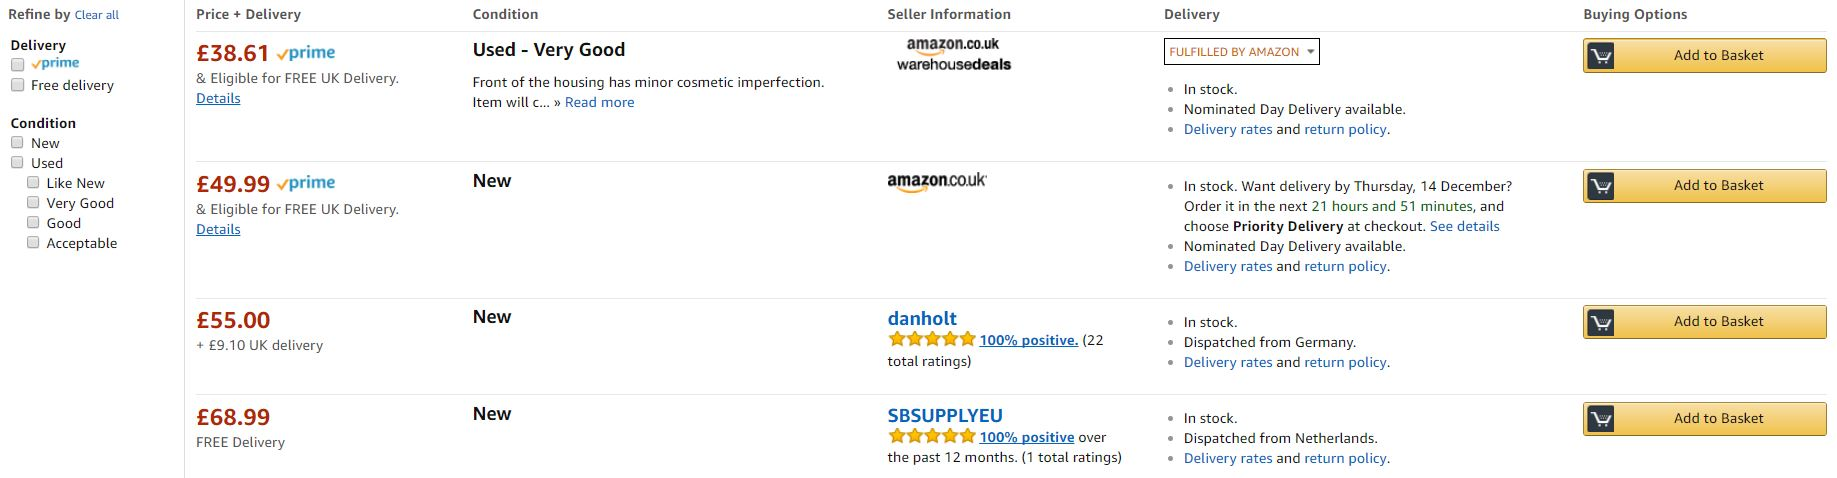
\includegraphics{fig2_offers.JPG}}
	\end{center}
	\caption{\label{fig:exampleoffer}An example of the offers for one product item on Amazon with many different competitors.}
\end{figure}

%\subsection{Data Understanding}
%\label{sec:DataUnderstanding}

%% how to get data?
\subsection{Amazon Web Service (AWS)}
\label{sec:awsData}
%% definition
 Amazon offers an array of tools to help sellers manage product selling. The most knowing of these tools is the Amazon Marketplace Web Service (MWS). Amazon Web Services (AWS) is a bundled remote computing service that provides cloud computing infrastructure over the Internet with storage, bandwidth and customized support for application programming interfaces (API).

From AWS, users has a capability to control their product updates for specified products from the Amazon cloud service. They are able to acknowledge their current state in the price-battle competed to their competitors. They can know who is the buy box winner, how many offers are provided by their competitors ... They also can execute several tasks through the provided functions such as listing products, managing inventory, and changing prices. 

The data from AWS can be pulled using the XML format, and then it can be parsed and stored into comma-separated value (CSV) file. Each row in the CSV file is a single data record or observation of one seller in the product's competition. Each column in the CSV contains a attribute of offers. 
%Its value is manually set by the seller or it is automatic defined by Amazon.

For example, \textbf{Fig.\ref{fig:exampleCSV}} illustrates small vision of one CSV file
which has four sellers, each in its own row. This observation contains 21 attributes, and some of them are very important such as \textit{IsBuyBoxWinner, ListingPrice, ShippingPrice, ShippingTime\_maxHours, ShippingTime\_minHours, IsFulfilledByAmazon}, ... In order to reduce the space, the description of features are skipped here. However, they can be briefly found in \textbf{Chapter \ref{sec:datafirstlook}}.

\begin{figure}[!h]
	\begin{center}
		\scalebox{0.5}{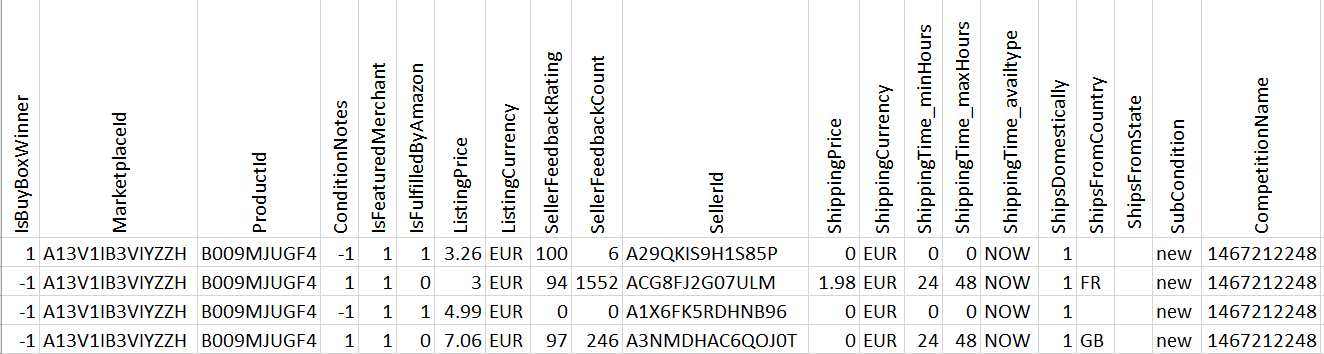
\includegraphics{exampleCSV.png}}
	\end{center}
	\caption{\label{fig:exampleCSV}An example of Amazon's data with 7 samples.}
\end{figure}

\subsection{Competition Auction}
\label{sec:amzAuction}

From mentioned above, the AWS helps users control their selling, including updating prices for their products. Whenever one seller changes or updates their offer for one item, AWS keeps a new record for that update with fully information for the lowest 20 prices offered of that product item (or less, if there are fewer than 20 offers). Since one auction happens, then one new XML is created from AWS.
